\chapter{Dataset}
\label{ch:dataset}
In this chapter we will describe in detail our simulations and our best strategy to do the automated temperature fitting. In the last section, we discuss the dataset obtained by this fitting.
\section{EPOCH Simulations}
The EPOCH simulation was run with the following parameters:
\begin{itemize}
	\item The laser wavelength is 1 micron.
	\item The laser is p-polarized and focused to a Gaussian spot of size $3.2$ mircons.
	\item The density in the target ranges from about $0.01n_c$ to $3.\gamma_{osc}n_c$, where $n_c$ is critical density corresponding to the laser radiation \cite{cui2013} and $\gamma_{osc}$ is defined in \cite{cui2013}.
	\item The initial temperature of plasma is 100 eV.
	\item The target is composed of electrons and protons. They are represented by 30 macro-particles per cell.
	\item The resolution of spatial grid is 33nm and the time step satisfies the CFL condition \cite{arber2015}.
	\item The intensities of the laser: $I=10^{17}\,\mathrm{W.cm}^{-2}$, $I=10^{18} \,\mathrm{W.cm}^{-2}$ and \newline$I=10^{19}\,\mathrm{W.cm}^{-2}$.
	\item The angle of incidence with respect to target normal direction: \newline $\alpha \in \{0\degree,1\degree,2\degree,3\degree,4\degree,5\degree,10\degree,20\degree,30\degree,40\degree,45\degree,50\degree,60\degree\}$.
	\item The characteristic scale length of the preplasma with exponential profile: \newline $L\in\{0.01,0.02,0.05,0.1,0.2,0.5,1,2,5\}$ in microns.
	
\end{itemize}
The simulations have been performed on the Q3 node of the Quantum Hyperion cluster at FNSPE. The input file that used to start the EPOCH simulation can be seen in appendix \ref{att:input-deck}. Hot electrons propagating into the target are recorded when they cross a virtual boundary inside the dense part of the target close to its rear side.

\section{Temperature fitting}
The results of the simulations are transformed into histograms as it was described in the beginning of chapter \ref{ch:temp-fitting-theory}. We fixed the energy histogram size to 1000 bins with their width scaling with the maximum electron energy. In the following pages, we will describe a strategy we developed and used to find the temperature from the vast majority of the energy histograms. The effectiveness of this strategy varies for different histograms, because it depends on multiple properties.

To get the best possible hot electron temperature fit, three things are important. First, because of the imperfections of the histogram related to the beginning and the end of the energy spectrum, it is helpful to narrow down the fitted region. Secondly, it is still necessary to perform a good fit automatically ideally without many issues. Last but not least, the fitting strategy has to be able to deal with the fact that the energy range and temperatures can for different histograms from the same dataset vary by several orders of magnitude. We will now present the two strategies developed for the purpose of this thesis and compare their performance.


\subsection*{Data preparation}
Before fitting the data, it is essential to prepare it appropriately. In practice, this involves removing a few bins in the beginning of the electron energy spectrum. The lower energy bins can be affected by error, as the low energy electrons need more time to reach the virtual detector and the simulation can end before that happens. Another reason, why this part of the distribution may be affected by error is the fact that these low energy electrons are more collisional and our simulations do not take collisions into account. Also, we made an approximation by considering Boltzmann distribution which does not work for small energies very well. Cutting the beginning is therefore justified. 

We also cut the end of the spectrum for reasons discussed in Chapter \ref{ch:temp-fitting-theory}. We cut it in a place where there is a first empty bin. Apart from the main reason, it is also not practical to work with empty bins in the logarithmically transformed version of the histogram. In special cases, it might be possible to work with histograms cut with less strict approach. However, these cut-offs help the analysis to focus on the relevant parts of the spectrum.


\begin{figure}[h]
	\centering
		\begin{subfigure}{0.49\textwidth}
		\centering
		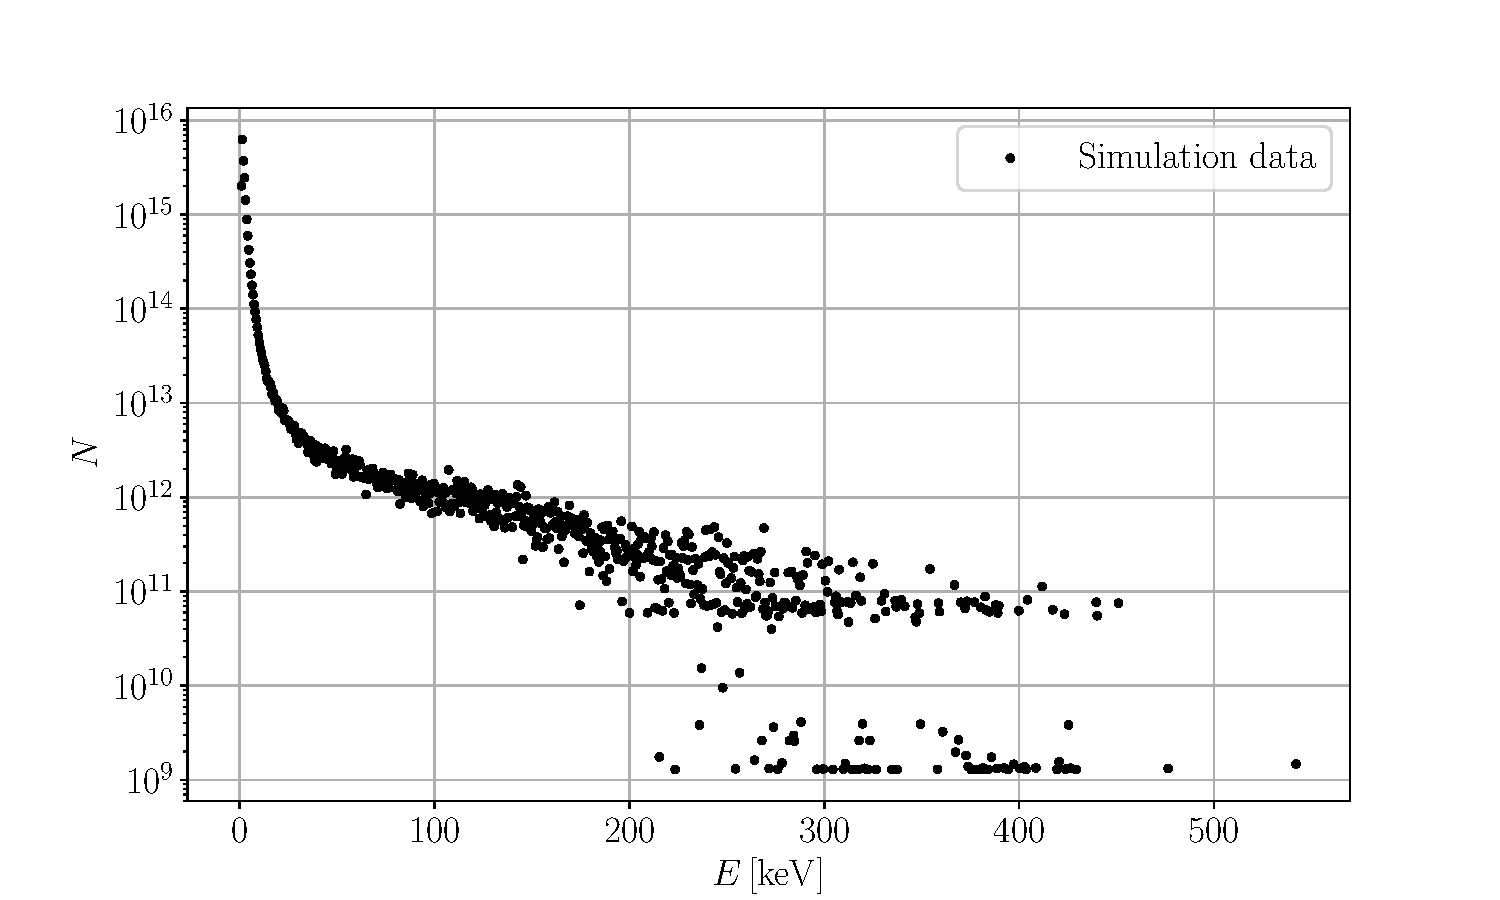
\includegraphics[width=\textwidth]{figures/untrimmed-hist}
		\caption{An example of uncut histogram.}
		\label{fig:ex-uncut}
	\end{subfigure}
	\hfill
	\begin{subfigure}{0.49\textwidth}
		\centering
		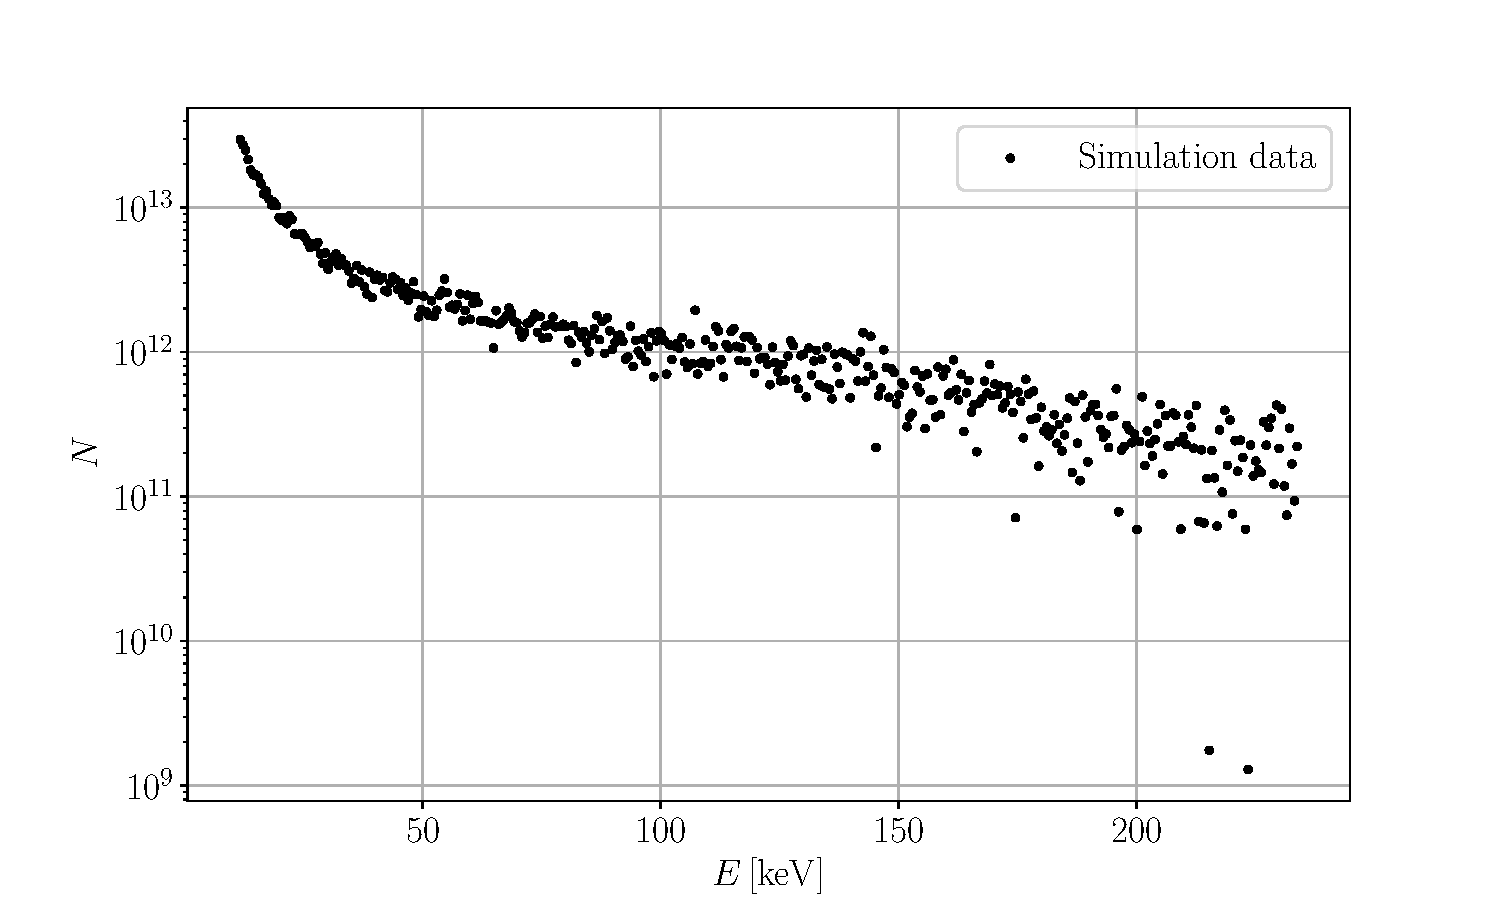
\includegraphics[width=\textwidth]{figures/trimmed-hist}
		\caption{An example of cut histogram.}
		\label{fig:ex-cut}
	\end{subfigure}
	\caption{Examples of histograms obtained with simulation parameters $I=10^{17}\,\mathrm{W.cm}^{-2}$, $L=1.0\,\mathrm{\mu m}$ and $\alpha = 30$°.}
	\label{fig:trimmed-hist}
\end{figure}

Examples of the uncut and cut histogram can be seen in figure \ref{fig:trimmed-hist}. Notice that the data show non-symmetrical noise in the part of the spectrum with the highest energies. This can be attributed to the logarithmic scale which can skew and seemingly magnify the noise for lower electron counts. 

For the purpose of the fitting, it is suitable to approximate the histogram data as points with $x$ values equal to the centre of the corresponding histogram bin and $y$ value equal to count.

\subsection*{Fitting method - Jacquelin}

The Jacquelin method for exponential parameter estimation was implemented in Python programming language as a class with number of exponential terms as a parameter. However, the lack of the numerical stability usually causes issues for more than three terms because of reasons discussed at the end of Chapter \ref{ch:temp-fitting-theory}. One can also choose whether the constant term should be included.

We found, that the majority of the histograms can be fitted by the three-exponential Jacquelin method without the constant term. Even though some histograms do not have three distributions present, the fit usually does not fail and the distribution corresponding to hot electrons can be (roughly) identified. Two examples of the three-exponential Jacquelin fit can be seen in Figures \ref{fig:3exp-fit-good-example}. We also highlighted the fitted hot electron (Boltzmann) distribution extracted from the fit.

\begin{figure}[ht]
	\centering
	\begin{subfigure}{0.49\textwidth}
		\centering
		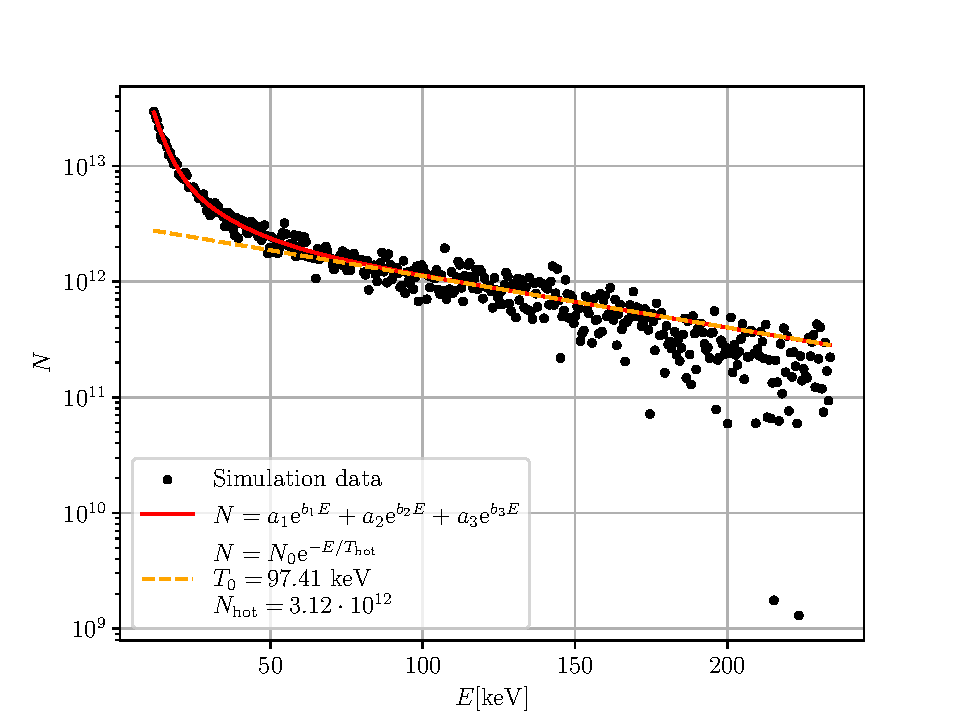
\includegraphics[width=\textwidth]{figures/3exp-ex1}
		\caption{An example of histogram obtained with simulation parameters $I=10^{17}\,\mathrm{W.cm}^{-2}$, $L=1.0\,\mathrm{\mu m}$ and $\alpha = 30$° fitted with the three-exponential Jacquelin method.}
		\label{fig:3exp-ex1-good}
	\end{subfigure}
	\hfill
	\begin{subfigure}{0.49\textwidth}
		\centering
		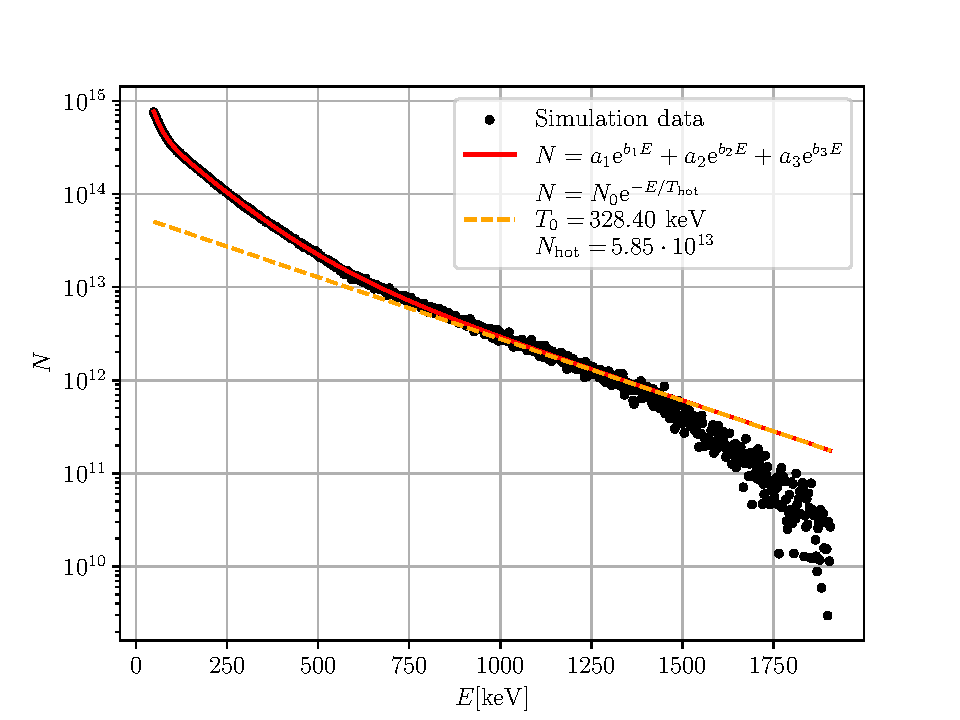
\includegraphics[width=\textwidth]{figures/3exp-ex2}
		\caption{An example of histogram obtained with simulation parameters $I=10^{19}\,\mathrm{W.cm}^{-2}$, $L=5.0\,\mathrm{\mu m}$ and $\alpha = 60$° fitted with the three-exponential Jacquelin method.}
		\label{fig:3exp-ex2-good}
	\end{subfigure}
	\caption{Three-exponential Jacquelin method fits.}
	\label{fig:3exp-fit-good-example}
\end{figure}

The hot electron temperature $T_\mathrm{hot}$ in Figure \ref{fig:3exp-fit-good-example} is calculated by:
\begin{equation}
	\label{eq:t-hot-from-b}
	T_{\mathrm{hot}} = -\frac{1}{b_3},
\end{equation}
where $b_3$ is chosen as the smallest of the negative coefficients $b_1,\, b_2,\, b_3$ in absolute value. 

In some fits, the absolute value of one of the factors $a_i$ $(i=1..3)$ can be small. Then the corresponding $b_i$ can be positive without significant impact on the fitted section of the histogram. In the limit of energy going to infinity, this does not have a valid physical interpretation, but it still does not have to be a concern if the other two terms behave well. In the other cases of the fit failing altogether, it often helps to narrow down the energy range even more from both ends (e.g. by 5 to 10 bins from each side) and try it again. If the fit fails multiple times despite the narrowing, the histogram one should rather fit it differently.

At the first sight, the Jacquelin method gives promising results. Qualitative analysis is done later when we compare the results to the temperature estimates done manually. For various reasons, there are situations where the Jacquelin method does not perform very well. The most probable reasons are related to irregularities at the end of the spectra where the energies do not seem to be very reliable. We noticed that this is especially the case for histograms from simulations run with intensity $I=10^{19}\,\mathrm{W.cm}^{-2}$. This also means that higher temperature estimates usually have a bigger chance to have larger error.

A graph with an example of a poor fit can be seen in Figure \ref{fig:3exp-ex-bad}. However, the fit is poor only when it comes to the hot electron temperature. One can immediately see that the $T_\mathrm{hot}$ estimate does not correspond to any part of the spectrum. The lower energy part of the spectrum are fitted well.
\begin{figure}[ht]
	\centering
		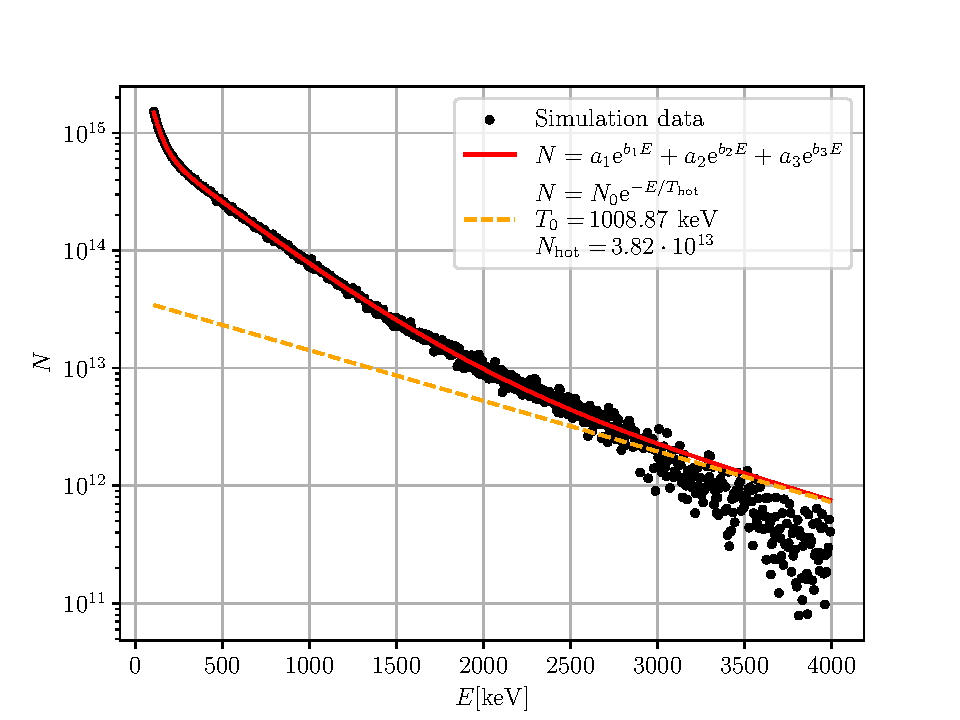
\includegraphics[width=0.8\textwidth]{figures/3exp-ex-bad}
		\caption{An example of histogram obtained with simulation parameters $I=10^{19}\,\mathrm{W.cm}^{-2}$, $L=0.6\,\mathrm{\mu m}$ and $\alpha = 30$° not very well fitted with the three-exponential Jacquelin method.}
		\label{fig:3exp-ex-bad}
\end{figure}

The reader might be curious, why it is not beneficial to use a weighted variant of this method. The idea would be to create scenario where reduction of error for higher energies is prioritized. The weights can be for instance set equal to standard deviation estimated as using Poisson statistics $\sigma_i = 1/y_i$.
The Jacquelin method can be modified quite simply to achieve something like that and it is true that we would prefer the hot electron distribution to be fitted with the biggest precision. However, in practice, this modification does not help with the quality of the fits. Again, this is because the high energy regions tend to be a little faulty.

\subsection*{Fitting method - Scanning}
The second fitting method is called Scanning. Here we take a segment -- in our case 150 bins -- and fit it with one exponential function $N = a\mathrm{e}^{bE}$. This also can be done explicitly because after logarithmic transformation we get:
\begin{equation}
	\label{eq:lin-one-exp}
	\mathrm{ln}(N) = A + bE
\end{equation}
where $A = \mathrm{ln}(a)$. Equation \ref{eq:lin-one-exp} is a linear equation and can be solved using classic linear regression. Estimation of standard errors $\Delta A$ and $\Delta b$ is simply calculated from the covariance matrix.

We do this for every set of consecutive 150 bins in the histogram. For example for histogram with 900 bins (after the initial cuts), we have 750 individual linear regressions. After that, we select the one with the smallest value of $b$ in absolute value. The $T_\mathrm{hot}$ estimate is calculated as $T_\mathrm{hot}=-1/b$. Naturally, the corresponding $a$ is set equal to $N_0$ from the Boltzmann distribution. The standard error estimates for $T_\mathrm{hot}$ and $N_0$ are then:
\begin{equation}
	\Delta T_\mathrm{hot} = \frac{\Delta b}{b^2} =  \Delta b\cdot   T_\mathrm{hot}^2
\end{equation}
and
\begin{equation}
	\Delta N_0 = e^A\cdot \Delta A  =  \Delta A  \cdot a,
\end{equation}
which follows from the error propagation formula.

\begin{figure}[ht]
	\centering
	\begin{subfigure}{0.49\textwidth}
		\centering
		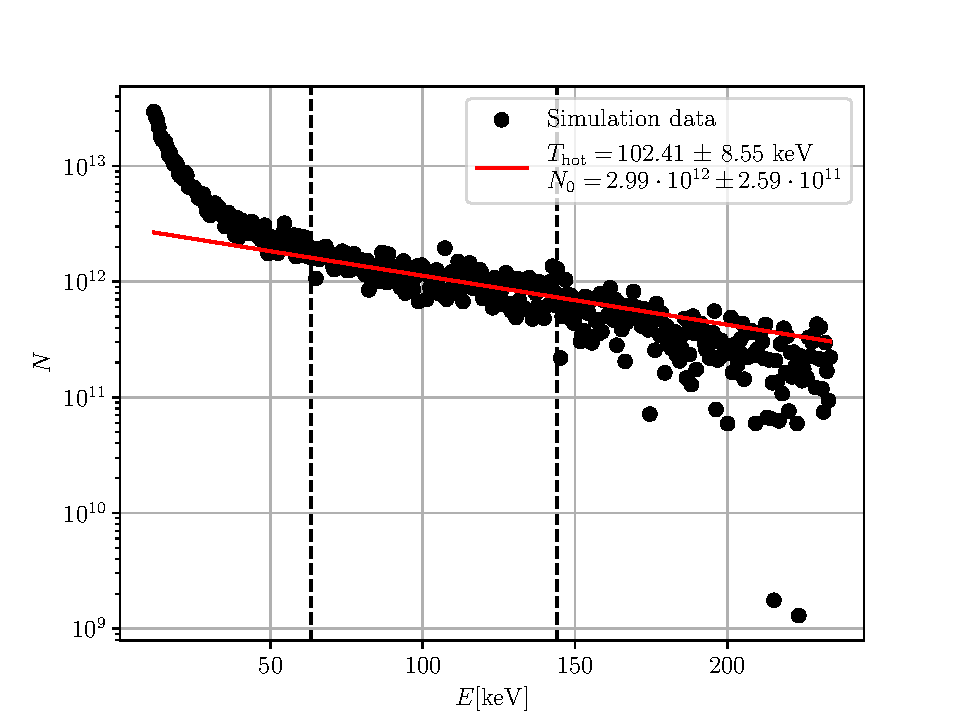
\includegraphics[width=\textwidth]{figures/scan-ex1}
		\caption{An example of histogram obtained with simulation parameters $I=10^{17}\,\mathrm{W.cm}^{-2}$, $L=1.0\,\mathrm{\mu m}$ and $\alpha = 30$° fitted with the Scanning method.}
		\label{fig:scan-ex1-good}
	\end{subfigure}
	\hfill
	\begin{subfigure}{0.49\textwidth}
		\centering
		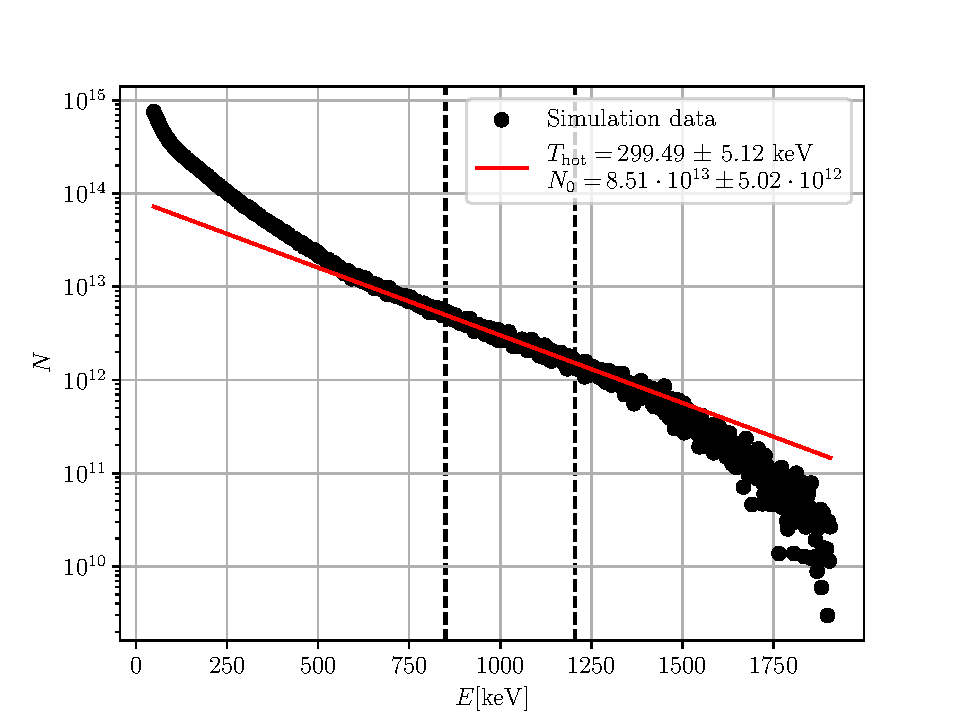
\includegraphics[width=\textwidth]{figures/scan-ex2}
		\caption{An example of histogram obtained with simulation parameters $I=10^{19}\,\mathrm{W.cm}^{-2}$, $L=5.0\,\mathrm{\mu m}$ and $\alpha = 60$° fitted with the Scanning method.}
		\label{fig:scan-ex2-good}
	\end{subfigure}
	\caption{Fit examples using the Scanning method.}
	\label{fig:scan-fit-good-example}
\end{figure}

Visually, this method seems to work very well. Two examples on the same histograms as before can be seen in Figure \ref{fig:scan-fit-good-example}. Here we also show two lines which show the start and the end of the fitted segment that produced fit with the highest temperature estimate. Estimates of $T_\mathrm{hot}$ and $N_0$ are very similar to results of the first method.

It is possible to fit a vast majority of our histograms using this method. The choice of how many bins one fits at a time obviously affects the results. The main factor by which one should decide is probably the initial number of bins. Generally, in this application, bigger fitted segments produce lower temperature estimates than smaller ones.

\subsection*{Fitting method - Manual}
As we said in the Chapter \ref{ch:temp-fitting-theory}, a tool was developed to make the manual fitting of $T_{\mathrm{hot}}$ and $N_0$ more effective. It was developed in Python using PyQt6 framework and it makes the manual fitting very quick for large amounts of histograms. Its effectiveness has roots in the possibility to load the whole folder with histograms and for each select the most reasonable region with two clicks of the mouse. The fit result is then saved directly to the dataset. We used a custom format to save the dataset so that it might be in the future extended to support different fitting strategies. Currently the only option is to select the range and click "Fit" which performs a linear regression in the same way as in the Scanning method. The tool also provides an option to show the original fit obtained by the automated process. 

An example of a fit performed manually can be seen in Figure \ref{fig:manual-fit-example}. The selected regions to be fitted are very similar to the automated selections of the previous method. 
\begin{figure}[ht]
	\centering
	\begin{subfigure}{0.49\textwidth}
		\centering
		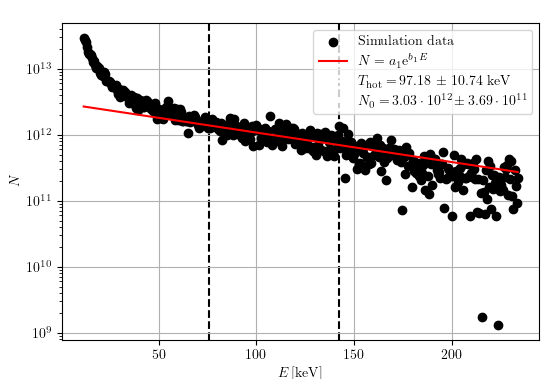
\includegraphics[width=\textwidth]{figures/hist_1e17_100_30_manual}
		\caption{An example of histogram obtained with simulation parameters $I=10^{17}\,\mathrm{W.cm}^{-2}$, $L=1.0\,\mathrm{\mu m}$ and $\alpha = 30$° fitted manually.}
		\label{fig:manual-ex1-good}
	\end{subfigure}
	\hfill
	\begin{subfigure}{0.49\textwidth}
		\centering
		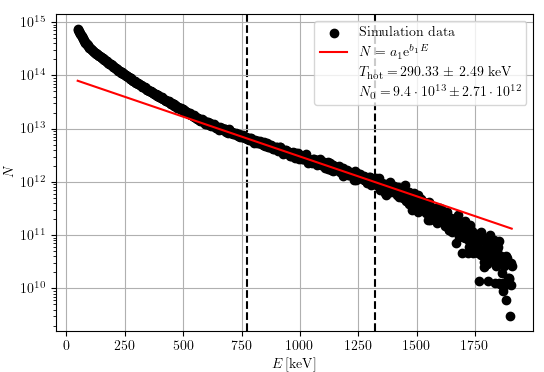
\includegraphics[width=\textwidth]{figures/hist_1e19_500_60_manual}
		\caption{An example of histogram obtained with simulation parameters $I=10^{19}\,\mathrm{W.cm}^{-2}$, $L=5.0\,\mathrm{\mu m}$ and $\alpha = 60$° fitted manually.}
		\label{fig:manual-ex2-good}
	\end{subfigure}
	\caption{Examples of manual fit for the same histograms as previously.}
	\label{fig:manual-fit-example}
\end{figure}


\subsection*{Comparison of the fitting strategies}
The comparison of the fitting strategies will be done in the following way. For each hot electron temperature estimate of the three-exponential Jacquelin method $T_\mathrm{hot,3exp}$ and the Scanning method $T_\mathrm{hot,scan}$ we calculate their relative error to the manual fit estimate $T_\mathrm{hot,manual}$ using:
\begin{equation}
	\mathrm{Relative \, error} = \frac{T_\mathrm{hot,3exp}-T_\mathrm{hot,manual}}{T_\mathrm{hot,manual}}
\end{equation}
and the same for $T_\mathrm{hot,scan}$. Then we calculate mean square relative error (MSRE) and mean absolute relative error (MARE) for both two methods. Before the averaging we throw away 40 worst fits for each method, because sometimes the estimate of the three-exponential fit is truly terrible and it would skew the results. Their values can be seen in Table \ref{tab:means_mses}. They may be a little unconventional metrics, but they still can give us a useful insight. 

\begin{table}[ht]
	\centering
	\caption{MSRE and MARE for fitting methods.}
	\begin{tabular}{lcc}
		\toprule
		Method & MSRE & MARE \\
		\midrule
		3exp  & 0.150 & 0.046 \\
		scan  & 0.110  & 0.019 \\
		\bottomrule
	\end{tabular}
	
	\label{tab:means_mses}
\end{table}

From the table, it is evident the Scanning method is better than the three-exponential Jacquelin method. Note that the MSRE is larger than MARE. Both metrics have values of the same order for both methods.

We plot the relative errors with respect to $T_\mathrm{hot,manual}$ for each evaluated simulation. The scatter plot containing the relative errors can be seen in Figure \ref{fig:relative-errors}. We again discard approximately 10 percent of fits - we put aside 20 worst 3-exp fits and then 20 worst Scanning fits of what remained to make the plot more compact. From the graph, we can conclude that the majority of the $T_\mathrm{hot}$ estimates is within the relative error of 0.5. That is probably acceptable for small values of $T_\mathrm{hot}$ (up to 20 keV), because the absolute value of this error is not that significant. For higher energies, having relative error 0.5 is disappointing to say the least, but it again points to the fact that the automation of the fitting is very challenging. The three-exponential Jacquelin method seems to perform quite poorly for estimates of temperature higher than 400 keV.

\begin{figure}[t]
	\centering
	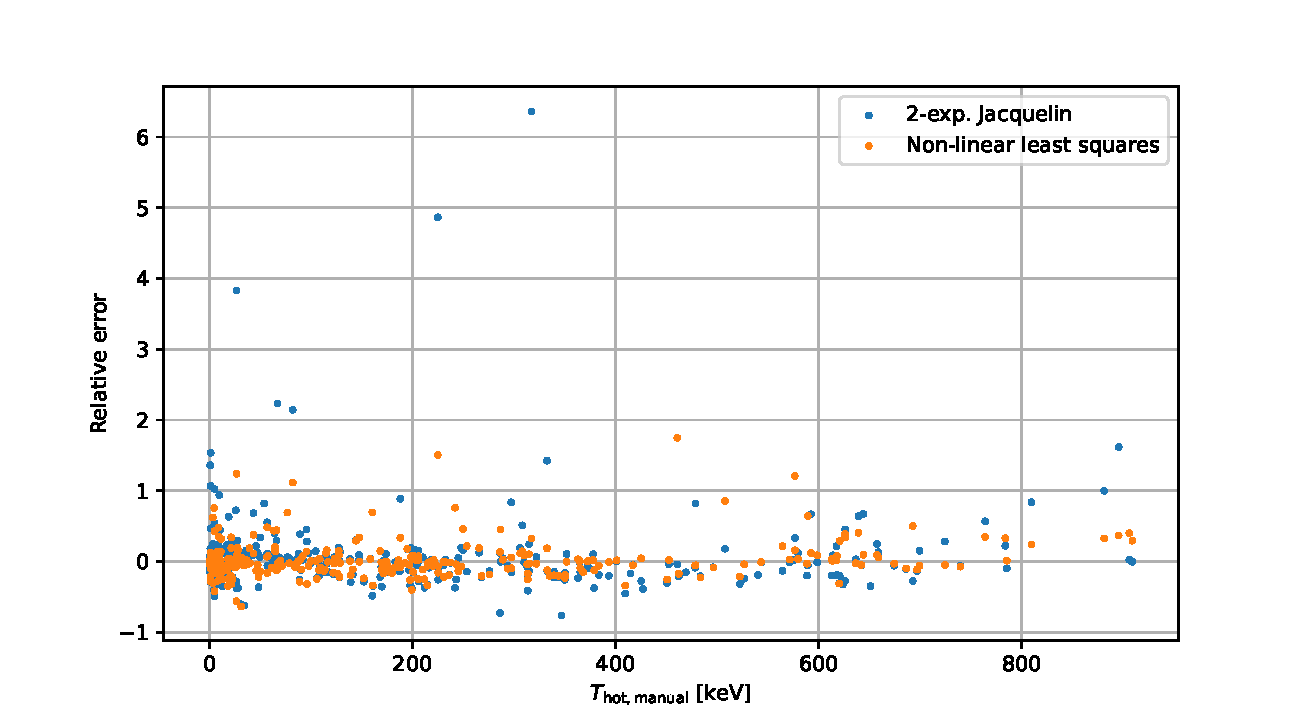
\includegraphics[width=0.98\textwidth]{figures/relative-error}
	\caption{Relative errors of the $T_\mathrm{hot}$ for two fitting methods.}
	\label{fig:relative-errors}
\end{figure}

The histograms of relative errors for both methods can be seen in Figure \ref{fig:relative-errors-hists}. It is possible to see that the three-exponential Jacquelin method has the relative errors much more symmetrical around 0 compared to the Scanning method. The systemic inaccuracy comes from the way we select the optimal fit. The strategy probably could be optimized if we took a different size of the histogram. However, making the fitted region larger can cause is to be larger than the actual region dominated by hot electrons in some histograms. One has to decide what is more important.

\begin{figure}[ht]
	\centering
	\begin{subfigure}{0.45\textwidth}
		\centering
		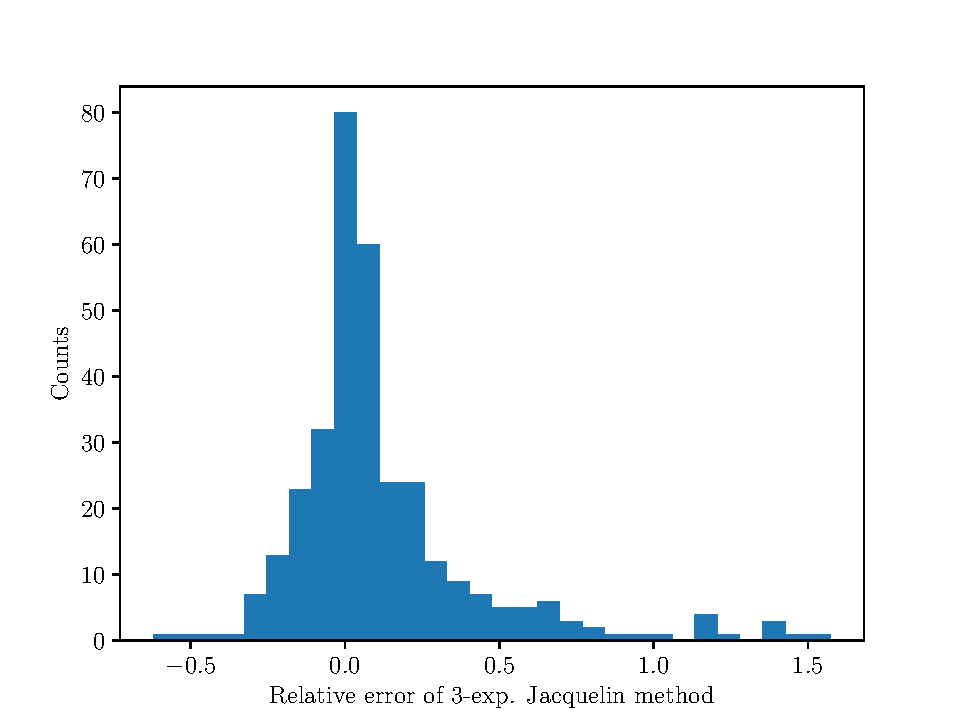
\includegraphics[width=\textwidth]{figures/3exp-residuals}
		\caption{3-exponential method relative errors.}
		\label{fig:3exp-histogram}
	\end{subfigure}
	\hfill
	\begin{subfigure}{0.45\textwidth}
		\centering
		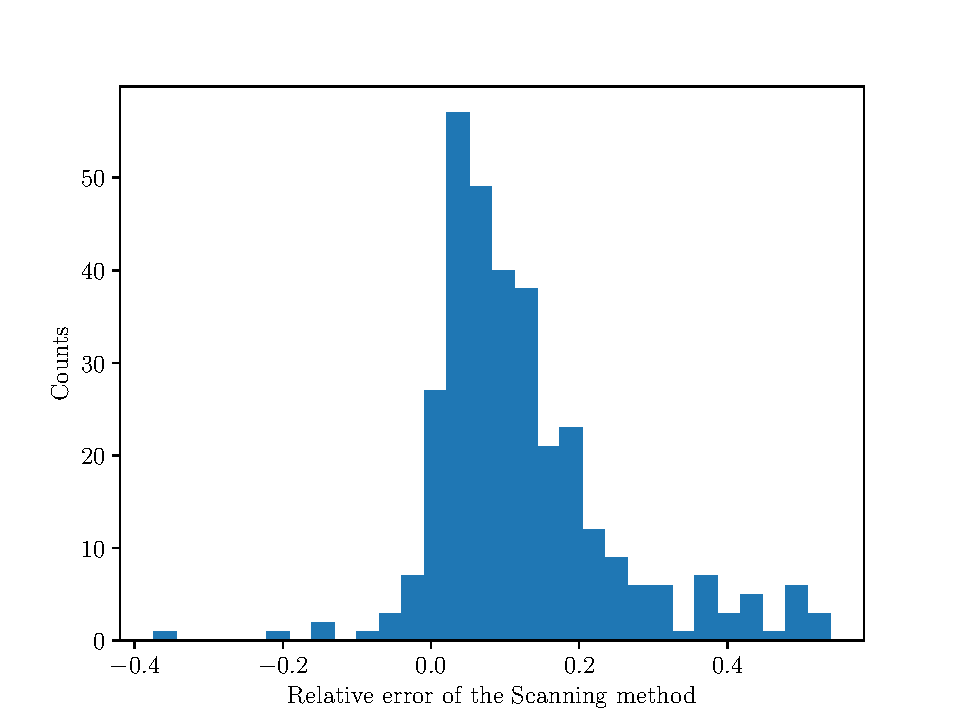
\includegraphics[width=\textwidth]{figures/scan-residuals}
		\caption{Scanning method relative errors.}
		\label{fig:scan-histogram}
	\end{subfigure}
	\caption{Relative errors from Figure \ref{fig:relative-errors} shown as histograms.}
	\label{fig:relative-errors-hists}
\end{figure}

It is difficult to say whether the $T_\mathrm{hot}$ estimates are good on their own. To get the idea, which histograms should be handled separately, we propose the following method. We take results from both strategies and find the relative difference (\textit{RD}) of the first one to the Scanning method defined intuitively as $RD_\mathrm{hot,scan} = \frac{T_\mathrm{hot,3exp}-T_\mathrm{hot,scan}}{T_\mathrm{hot,scan}}$.

We can plot these in a similar way as before but now with $T_\mathrm{hot,scan}$ on the bottom axis. The results can be seen if Figure \ref{fig:relative-errors-two}. There are multiple occasions where the three-exponential Jacquelin method produces too large estimates. Note that the largest values on $T_\mathrm{hot,scan}$ axis are larger than before. This corresponds to the positive relative errors for large $T_\mathrm{hot,manual}$ in Figure \ref{fig:relative-errors-two}.

\begin{figure}[h]
	\centering
	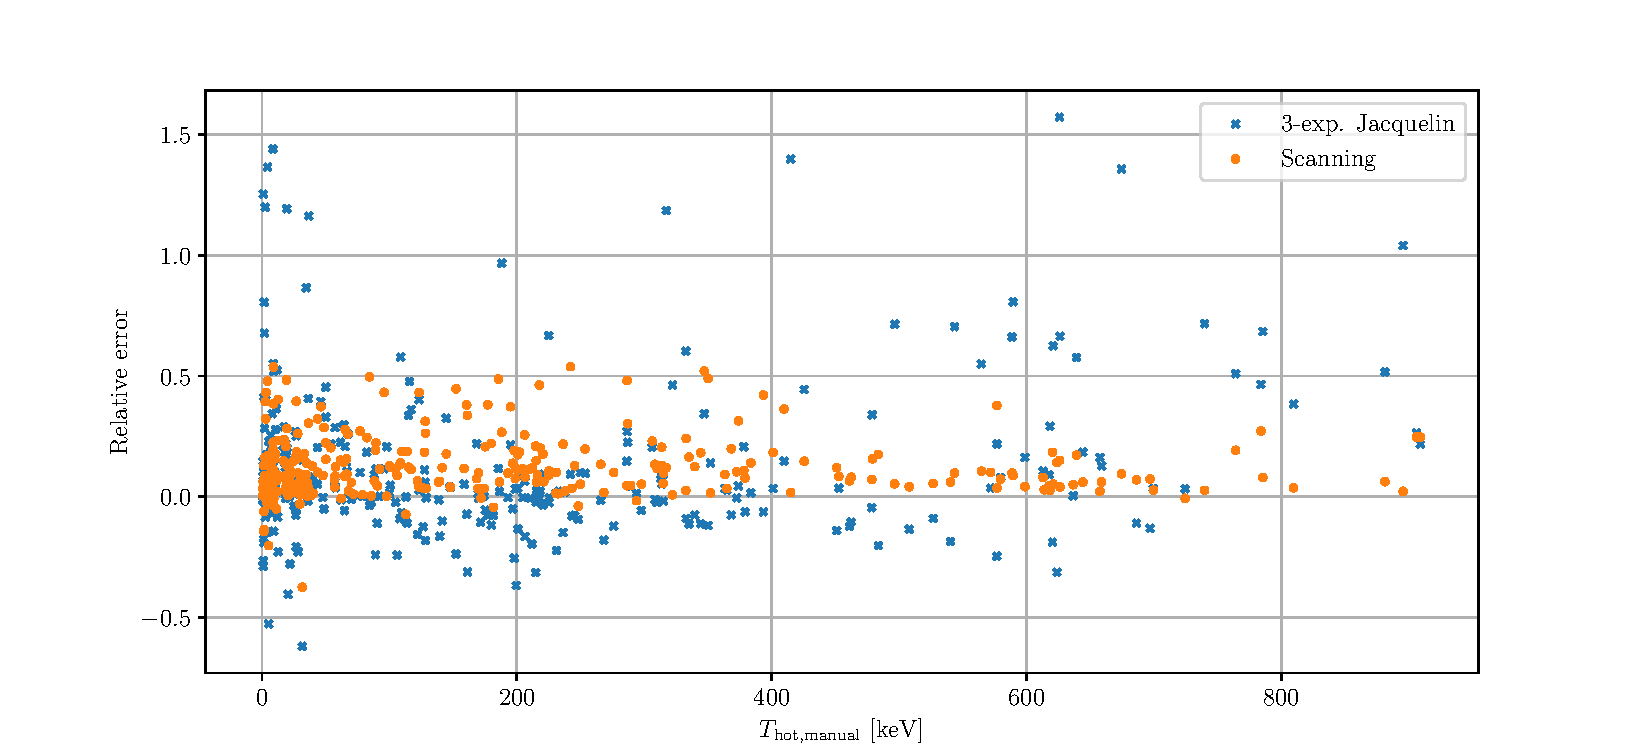
\includegraphics[width=0.98\textwidth]{figures/relative-error2}
	\caption{Relative errors of 3-exponential Jacquelin method with respect to Scanning method.}
	\label{fig:relative-errors-two}
\end{figure}

In cases where the difference is large, we should consider examining them manually, because the difference might suggest that the histogram is problematic. The selection of threshold for \textit{large} is a matter of trade-off between the time spent examining various histograms and the precision. What we proposed proves to be a good way of identifying the worst estimates first. It could be attributed to the fact that the methods are different and independent and the likelihood that both give absurd results is low.

In conclusion, we can say that there definitely is a necessity for improvement of the fitting, if one wants to rely on fitting thousands of histograms at once. The presented strategies can sometimes produce acceptable results and we have shown a mechanism for identifying the results with high uncertainty. However, in the current state, even the rest of the fits probably shouldn't be completely unsupervised. Without a brief inspection of each fitted histogram, the reliability can be questionable. Needless to say, both of the presented methods may serve as a starting point for further improvement.



\newpage
\section{Full dataset}
In this section, we will present the dataset used for modelling. Naturally, the results from 378 simulations contain a lot of information most of which will be discarded. As we concluded at the end of the previous section, the automation of the temperature fitting brings many challenges, some of which were not exhaustingly solved. From now on, we will be using the manually labelled dataset as such data are considered the most reliable. The main goal of this section is to visualize the interesting aspects of the data we obtained so far.
\begin{figure}[ht]
	\centering
	\begin{subfigure}{0.49\textwidth}
		\centering
		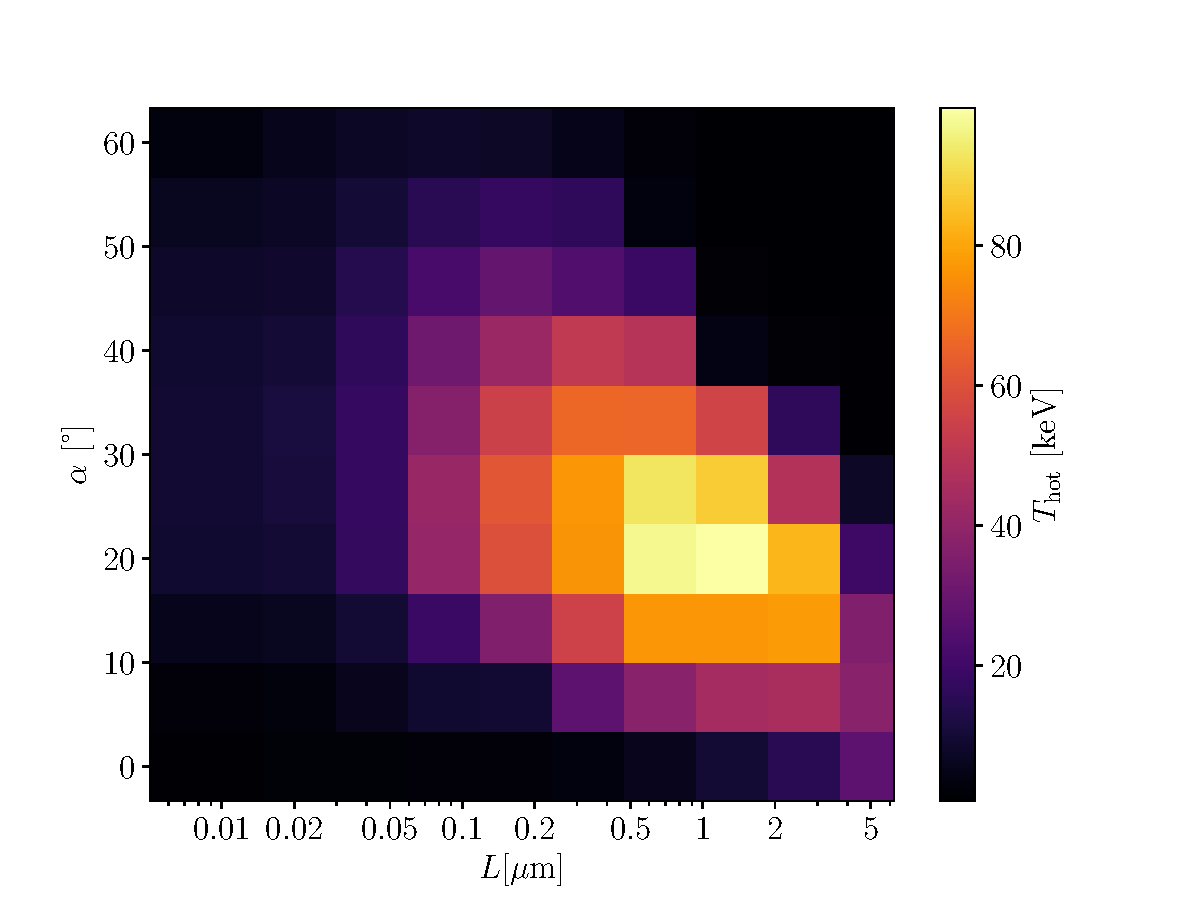
\includegraphics[width=\textwidth]{figures/I_1e17t_hot}
		\caption{Dataset with $I = 10^{17} \, \mathrm{W.cm}^{-2}$.}
		\label{fig:dataset1-a}
	\end{subfigure}
	\hfill
	\begin{subfigure}{0.49\textwidth}
		\centering
		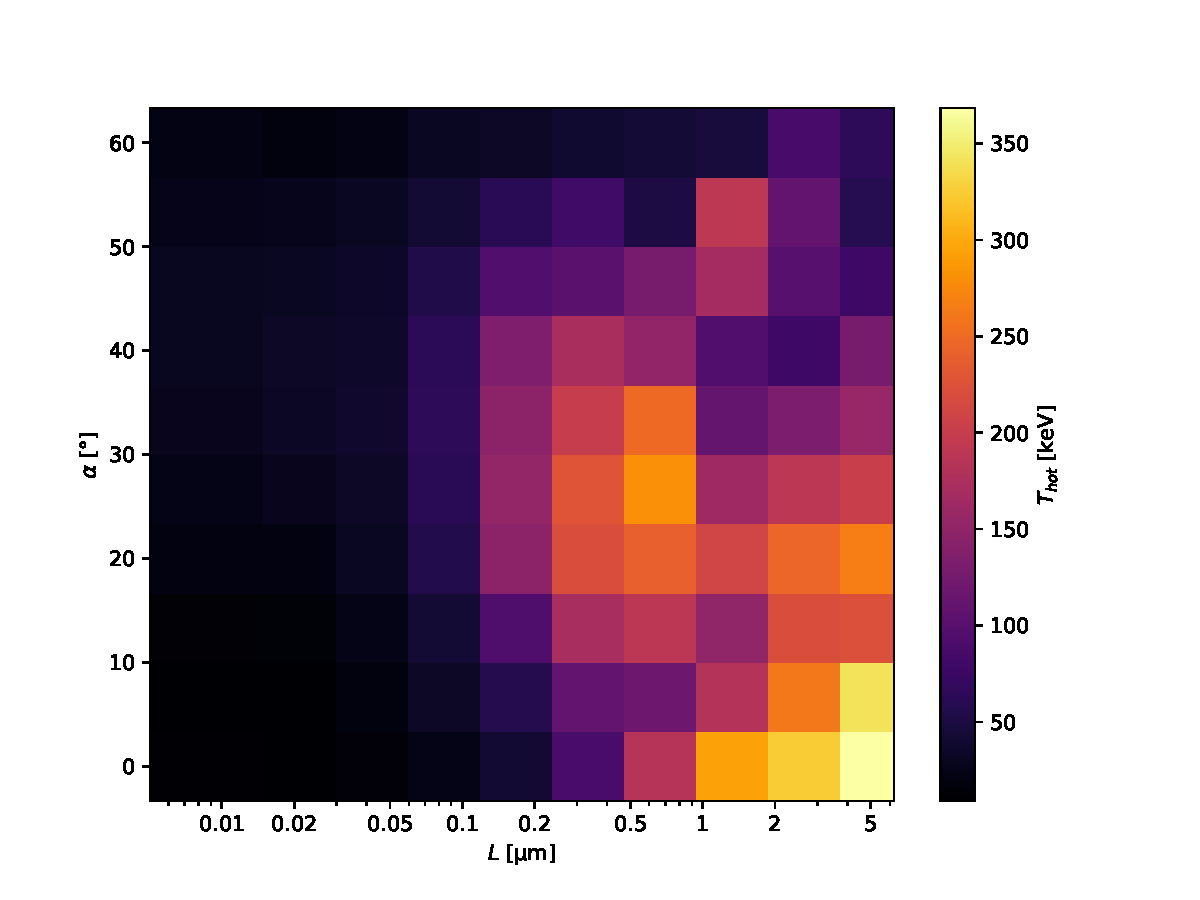
\includegraphics[width=\textwidth]{figures/I_1e18t_hot}
		\caption{Dataset with $I =  10^{18} \, \mathrm{W.cm}^{-2}$.}
		\label{fig:datset1-b}
	\end{subfigure}
	\begin{subfigure}{0.49\textwidth}
		\centering
		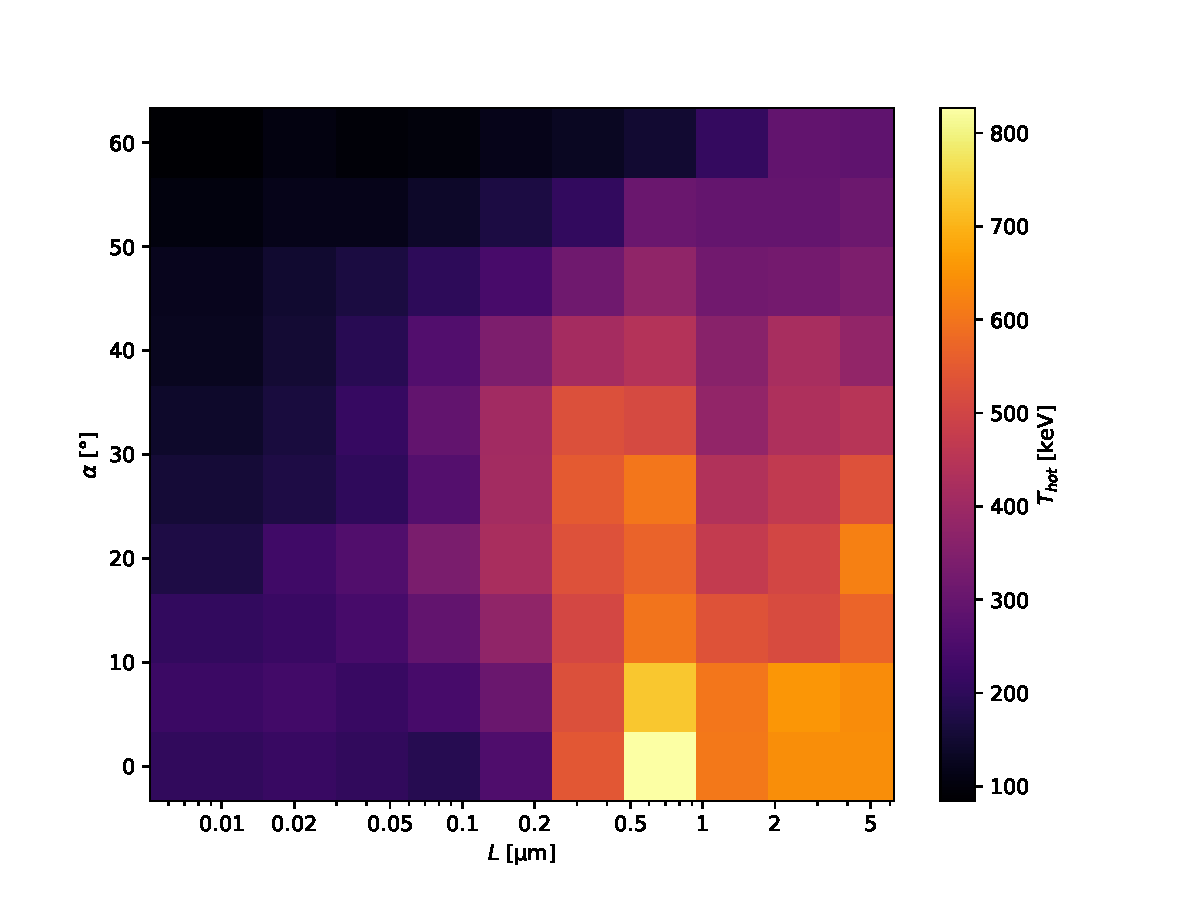
\includegraphics[width=\textwidth]{figures/I_1e19t_hot}
		\caption{Dataset with $I = 10^{19} \, \mathrm{W.cm}^{-2}$.}
		\label{fig:dataset1-c}
	\end{subfigure}
	\caption{Illustration of dataset shown for three simulated intensities.}
	\label{fig:dataset1}
\end{figure}


The visualization of the dataset itself can give us valuable insight to the behaviour of the function of $T_{\mathrm{hot}} = T_{\mathrm{hot}}(I,L,\alpha)$. Because there are three parameters for which $T_{\mathrm{hot}}$ is being modelled, the visualization can be tricky. The issue can be approached from multiple points of view.

Let us start by showing the dependency of the fitted temperature on simulation parameters with three fixed intensities $I = 10^{17} \,\mathrm{W.cm}^{-2}$, $I = 10^{18} \,\mathrm{W.cm}^{-2}$ and $I = 10^{19} \,\mathrm{W.cm}^{-2}$. This way we can "slice" through the three dimensional space of parameters and get a good idea what we are modelling. By the way, this approach is almost completely corresponding to the way the parameter space was sampled for the simulations. Most of the parameters were chosen as a points of grid with certain steps in $\alpha$ and logarithmic steps in $L$. This is not true for all points and because of that, these graphs were made using linear interpolation to the grid of similar density. In other words, the values should not be considered exact and the graphs serve only as illustration. The graphs can be seen in Figure \ref{fig:dataset1}.


The initial observation from these three graphs can for instance be the increasing temperature scales on the right side of each graph, which corresponds to the increasing intensity. This demonstrates the fundamental relationship: as the energy carried by the laser pulse increases, the temperature of the hot electrons rises too. Next thing one might notice is that size of the temperatures range also changes with intensity. For both $I = 10^{17}ň, \mathrm{W.cm}^{-2}$ and $I = 10^{18}ň, \mathrm{W.cm}^{-2}$, there is a region (or simulation point) with hot electron temperature close to zero. For intensity $I = 10^{19} ň,\mathrm{W.cm}^{-2}$ this region disappears. 

It is also possible to make some qualitative comments about the dataset in the light of the absorption theory which was briefly discussed in Chapter \ref{ch:plasma-theory}. For example, one might be the optimal angle of resonance absorption described by Equation \ref{eq:res-opt}. We claimed that the other absorption mechanism are expected to be most dominant for higher laser intensities. For intensity $I = 10^{17} \, \mathrm{W.cm}^{-2}$, we can find an agreement with this theoretical model by plotting the optimal resonance absorption curve on top of that part of the dataset. Such graph can be seen in Figure \ref{fig:opt-res-abs}.

\begin{figure}[t]
	\centering
	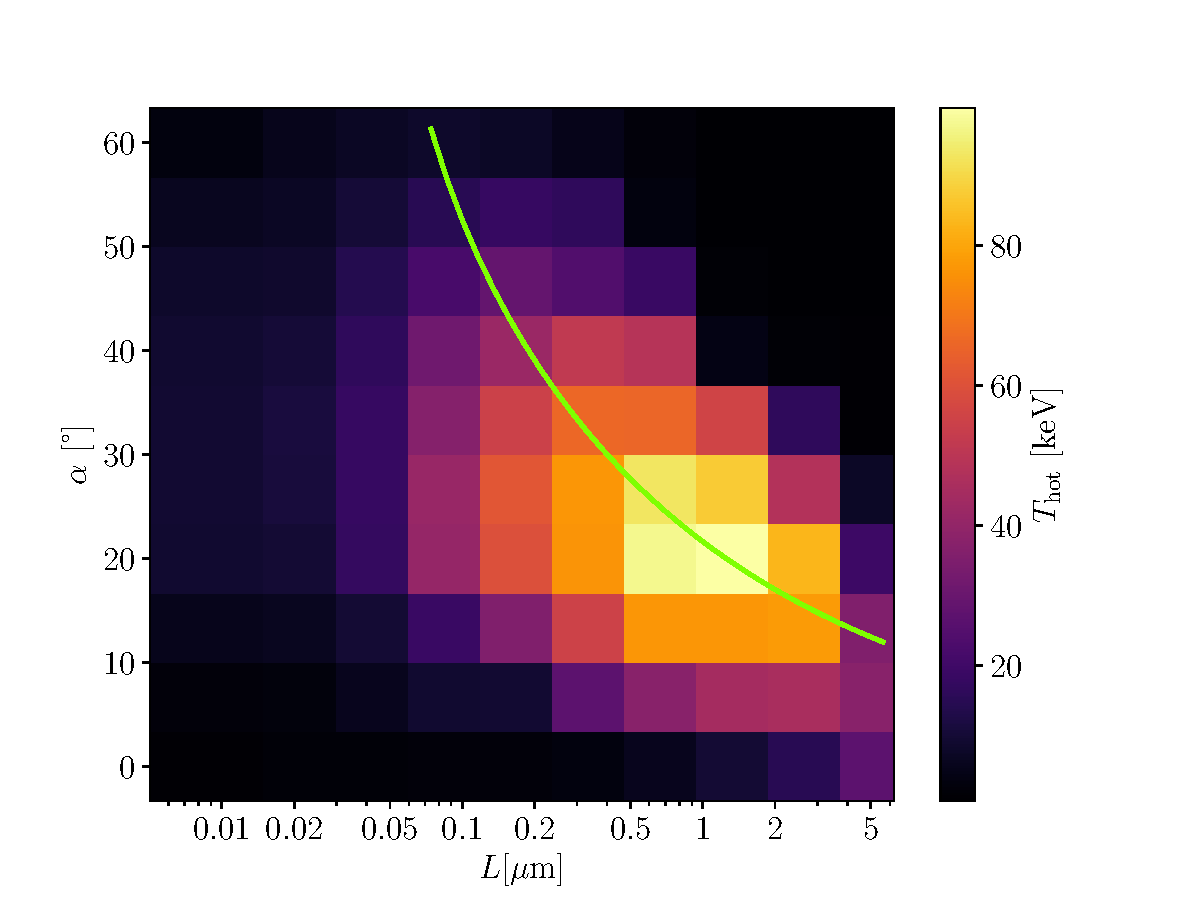
\includegraphics[width=0.60\textwidth]{figures/optimal-res-absorption}
	\caption{A part of dataset with $I = 10^{17} \, \mathrm{W.cm}^{-2}$ with optimal resonance absorption curve (the green curve).}
	\label{fig:opt-res-abs}
\end{figure}

On the other hand, for higher intensities there appears a different maximum for small angles and longer preplasma scale lengths. This agrees with theory about $\bm{J} \times \bm{B}$ heating.

What might be particularly interesting is the evident rise of temperatures for $L=0.5 \,\mathrm{\mu m}$ for the intensity $I = 10^{19}\, \mathrm{W.cm}^{-2}$, especially for small incidence angles. The total absorption is relatively small for these parameters, as can be seen in Figure~\ref{fig:dataset2-c}. In this case, the density scale length is equal to half the laser wavelength. This means that the standing wave which develops due to interference of the incident and the reflected laser wave exactly matches with the plasma density profile. This case requires further investigation which is beyond the scope of this thesis but it is inspired by these results.

It is important to realize, that these graphs do not represent the general absorption patterns. To compare \textit{total} absorption across the domain of simulation points, it is necessary to also include the energy absorbed by the rest of the electrons. We will visualize it in similar way but instead of temperature, we look at the overall energy carried by all the electrons. This can be done by integrating each of the histograms. For the same reasons as in the previous section, we restrict ourselves to electron energies higher than threshold of 10 keV. The total absorbed energy for the same three intensities is displayed in the graphs in Figure \ref{fig:dataset2}.

\begin{figure}[ht]
	\centering
	\begin{subfigure}{0.49\textwidth}
		\centering
		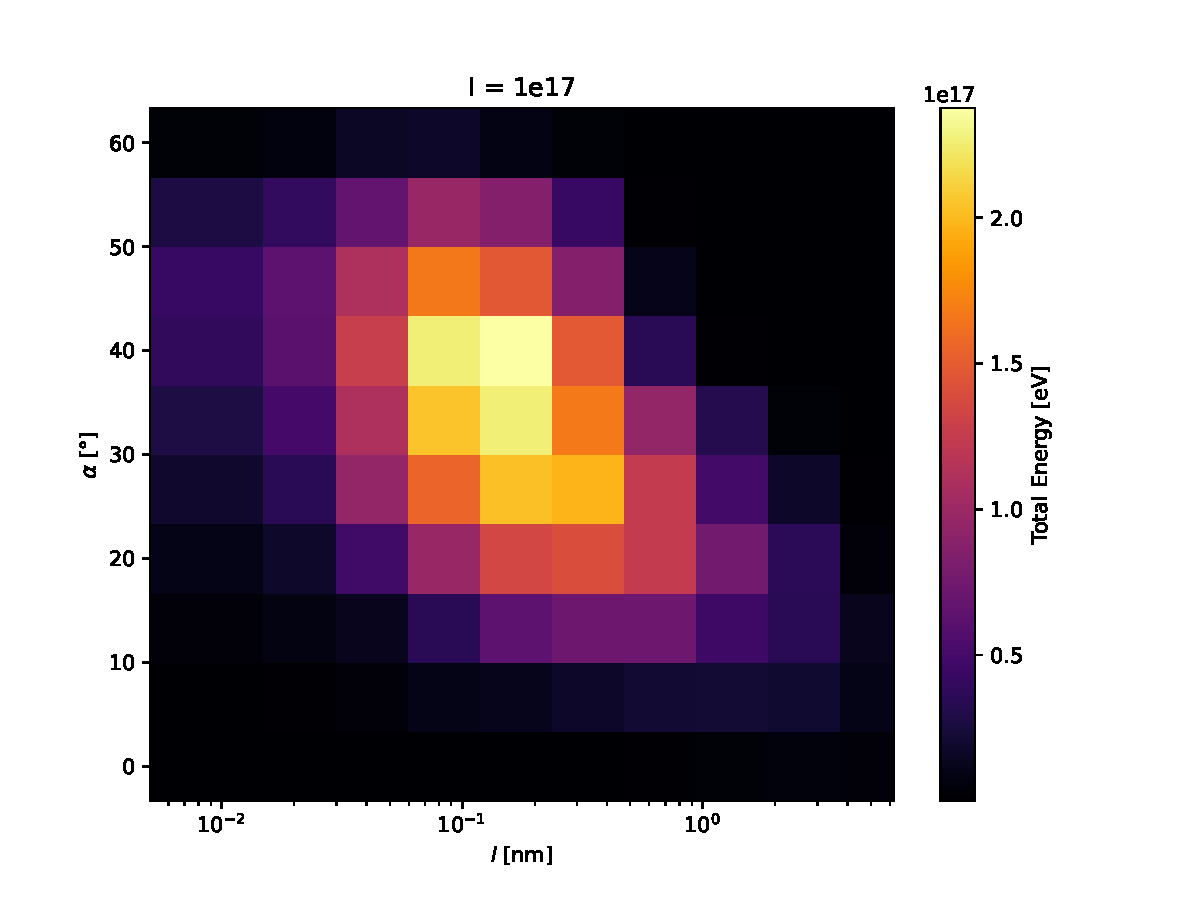
\includegraphics[width=\textwidth]{figures/I_1e17_cut_10}
		\caption{Dataset with $I = 10^{17} \, \mathrm{W.cm}^{-2}$.}
		\label{fig:dataset2-a}
	\end{subfigure}
	\hfill
	\begin{subfigure}{0.49\textwidth}
		\centering
		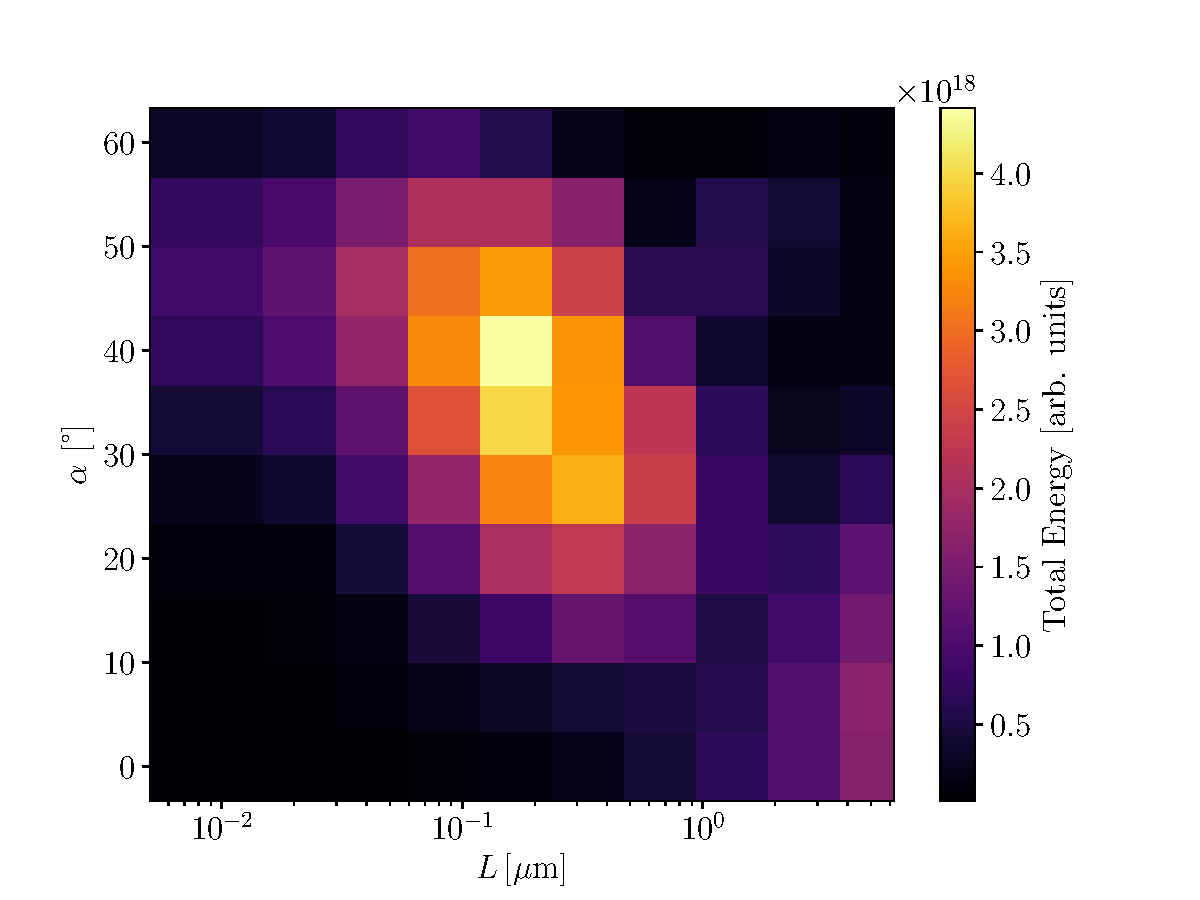
\includegraphics[width=\textwidth]{figures/I_1e18_cut_10}
		\caption{Dataset with $I =10^{18} \, \mathrm{W.cm}^{-2}$.}
		\label{fig:datset2-b}
	\end{subfigure}
	\begin{subfigure}{0.49\textwidth}
		\centering
		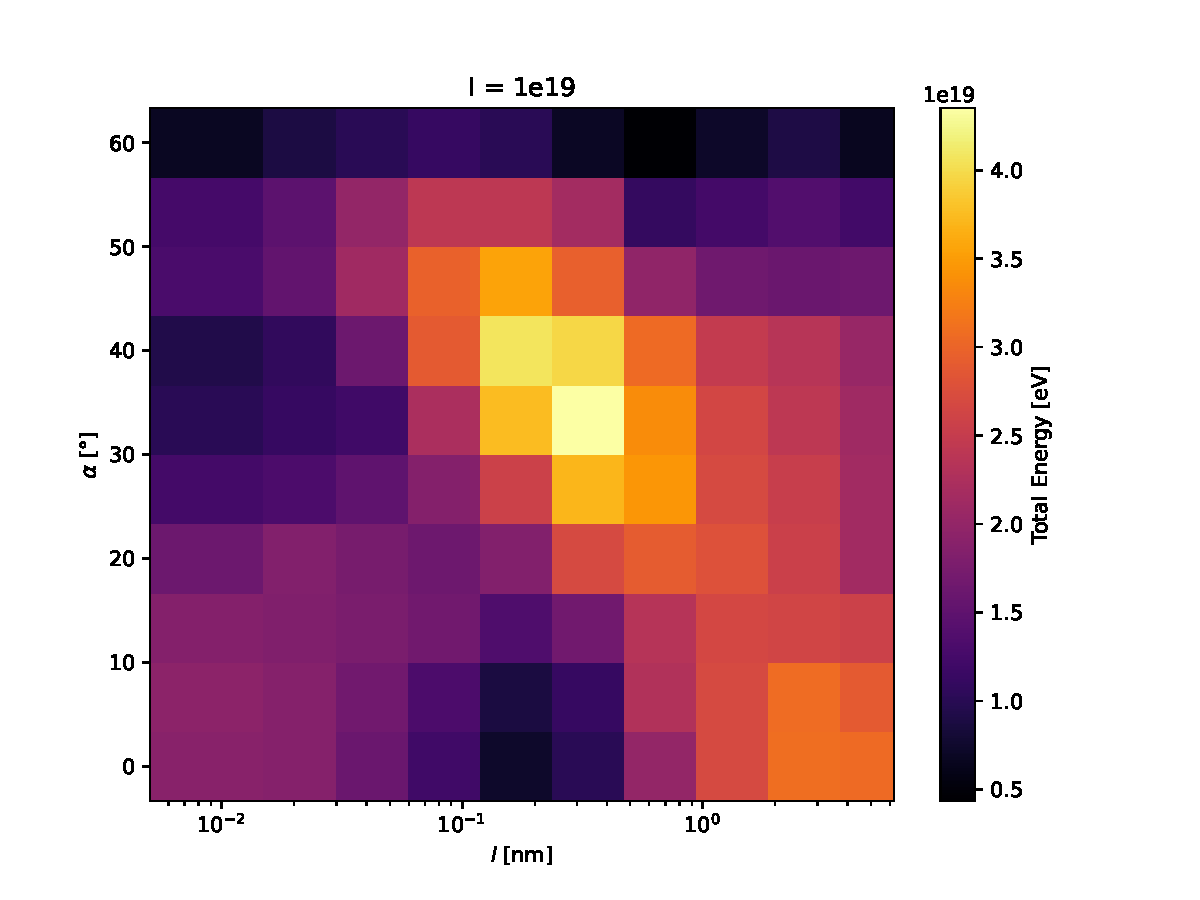
\includegraphics[width=\textwidth]{figures/I_1e19_cut_10}
		\caption{Dataset with $I = 10^{19} \, \mathrm{W.cm}^{-2}$.}
		\label{fig:dataset2-c}
	\end{subfigure}
	\caption{Illustration of total energy absorption shown for three simulated intensities.}
	\label{fig:dataset2}
\end{figure}

It is possible to see, that the maximum overall absorption is happening in cases of bigger incidence angles. As discussed before, the resonance absorption and vacuum heating both require a finite incidence angle which can be relatively large. Also for the intensity $I = 10^{19} \, \mathrm{W.cm}^{-2}$ there is relatively larger absorption happening for small angles and large scale lengths. This is in agreement with the theory presented in Chapter \ref{ch:plasma-theory}.

Moving on, let us shift our attention back to the study of the actual dataset of temperatures. Without interpolation, we can plot the temperature with respect to scale length and incidence angle so that the actual values of temperature are more clear. Three graphs corresponding	 to the same three intensities are shows in Figure~\ref{fig:dataset3}. We do not show all the simulated points (we skip the small angles), because it helps with the readability.

\begin{figure}[t]
	\centering
	\begin{subfigure}{0.49\textwidth}
		\centering
		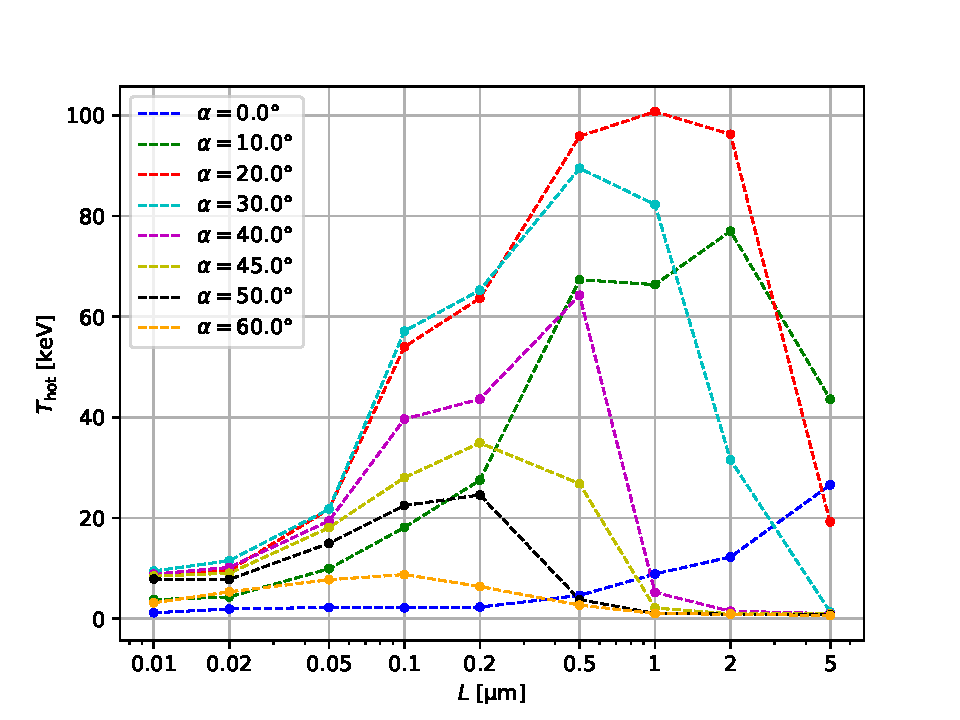
\includegraphics[width=\textwidth]{figures/t_hot_l_17}
		\caption{Dataset with $I = 1 \times 10^{17} \mathrm{W.cm}^{-2}$.}
		\label{fig:dataset3-a}
	\end{subfigure}
	\hfill
	\begin{subfigure}{0.49\textwidth}
		\centering
		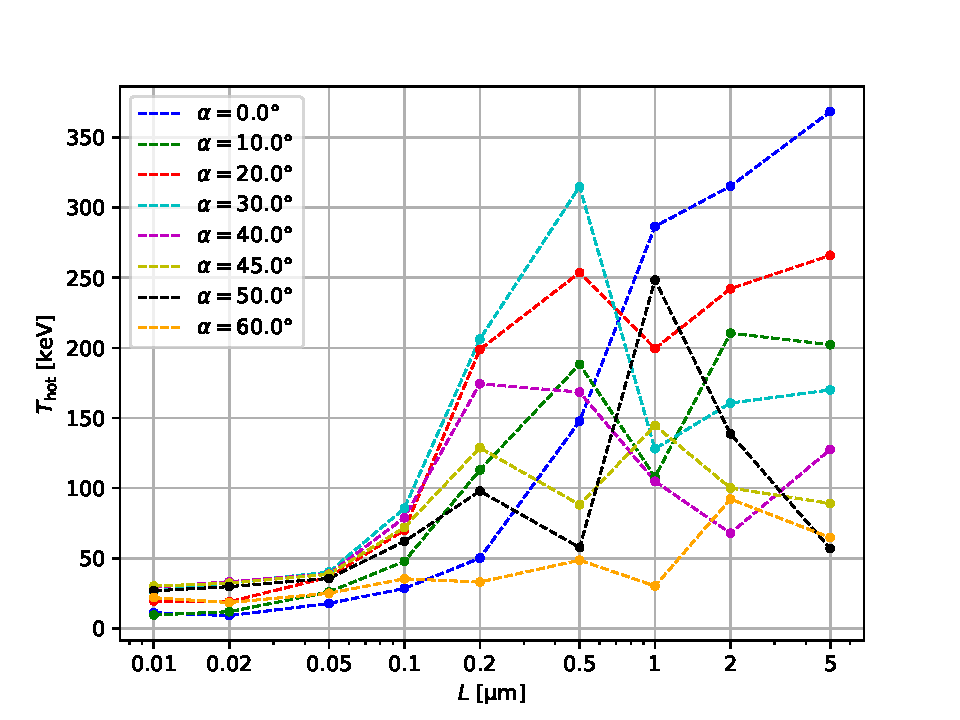
\includegraphics[width=\textwidth]{figures/t_hot_l_18}
		\caption{Dataset with $I = 1 \times 10^{18} \mathrm{W.cm}^{-2}$.}
		\label{fig:datset3-b}
	\end{subfigure}
	\begin{subfigure}{0.59\textwidth}
		\centering
		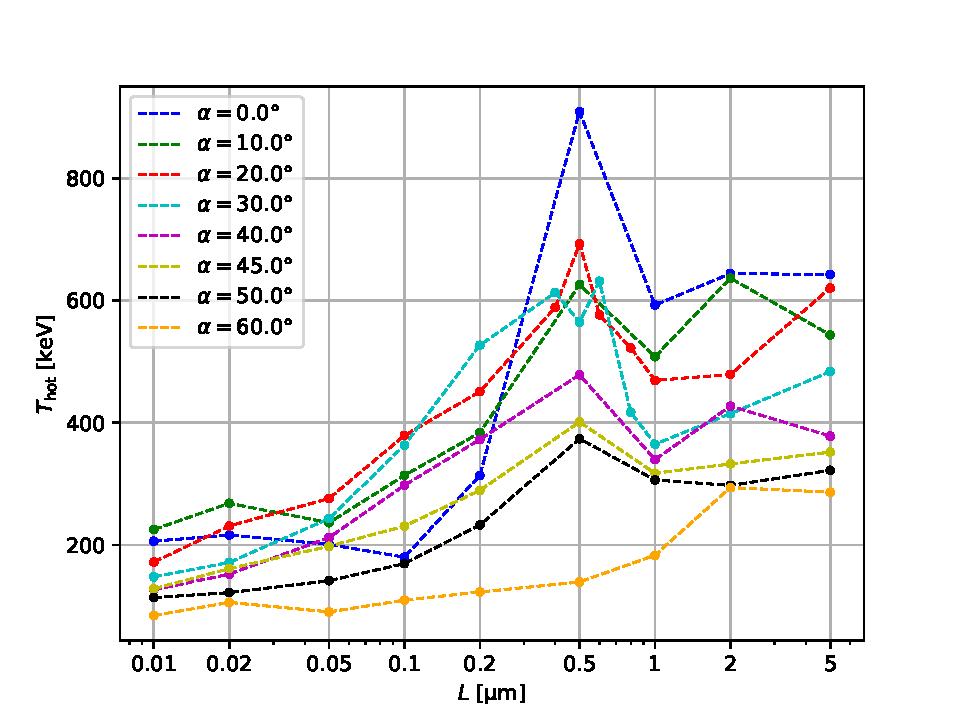
\includegraphics[width=\textwidth]{figures/t_hot_l_19}
		\caption{Dataset with $I = 1 \times 10^{19} \mathrm{W.cm}^{-2}$.}
		\label{fig:dataset3-c}
	\end{subfigure}
	\caption{Dataset for three simulated intensities shown in different axes.}
	\label{fig:dataset3}
\end{figure}

